\section{Measurement Strategy}\label{s:measurement}
\cut{
\begin{outline}
\1 Packet marking for hands-off measurement
    \2 Congestion control protocols require accurate measurements for their decisions to be meaningful. How can an inbox and outbox collaborate to measure network conditions along their path?
    \2 Congestion control protocols need only a small, common set of measurements~\cite{ccp-hotnets} to function. We observe that these can be reconstructed with three core measurements: the sending rate at the in-box, the receiving rate at the out-box, and the round-trip time between the two gateways.
    \2 Unfortunately, to be most useful, the sending and receiving rates should be calculated over the same set of packets. Otherwise \an{why}.
        \3 Otherwise instantaneous measurements can't be used and everything has to be ewma'd?
    \2 We use packet flagging to synchronize these measurement epochs between the sender and the receiver.
    \2 Packet flagging is a technique where the inbox and outbox agree on some desired epoch length in packets.
    \2 Then, the inbox takes the hash of some field in the packet header (\eg TCP sequence number or IP ID).   
        \3 A suitable field should change with every packet (\ie, is not static for the lifetime of the connection).
        \3 On every packet p, given a desired epoch duration d, the inbox computes x = H(p) mod d where H is some hash function (which need not be cryptographically secure)
    \2 Epoch-based measurements
        \3 The inbox checks if x == 0. If it is, the inbox marks the start of a new epoch. It records the current time, and the cumulative number of bytes sent since some previous super-epoch.
        \3 Similarly, the outbox computes x = H(p) mod d on every packet. On a packet marking the start of a new epoch, the outbox sends an out-of-band packet to the inbox containing the hash of the epoch-marked packet, its current time, and the cumulative number of received bytes sent since the super-epoch.
        \3 When the inbox receives an out-of-band feedback message, it looks up that hash. If the packet which ended the previous epoch was sent at time $s_1$ and received at $r_1$, and the packet ending the current epoch was sent at time $s_2$ and received at $r_2$, the inbox can calculate:
            \4 rtt = current time - $s_2$
            \4 bytes in send epoch = bytes sent at s2 - bytes sent at s1
            \4 bytes in recv epoch = bytes sent at r2 - bytes sent at r1
            \4 send epoch duration = r2 - r1
            \4 received rate = bytes in recv epoch / recv epoch duration
        \3 Epoch durations are in expectation, since they depend on hash values.
    \2 The inbox now has relevant measurements, and can compute estimates of higher-level measurement primitives.
        \3 \eg loss rate = send rate - recv rate
\1 Suitable congestion control algorithms
    \2 Since \name cannot track low-level metrics used by traditional congestion control algorithms such as the number of inflight packets, implementations of window-based algorithms may not be suitable for use.
    \2 Fortunately there are rate-based algorithms available~\cite{bbr, nimbus}.
    \2 The inbox acts as a datapath for CCP~\cite{ccp}, and we use CCP implementations of BBR and Nimbus without modification.
\end{outline}
\fi
}

In this section we describe how the \inbox and \outbox can coordinate to compute accurate and robust
measurements of the network conditions necessary for congestion control.

Prior work has shown that congestion control algorithms typically need only a small, common
set of measurements~\cite{ccp-hotnets} to function. In particular, rate-based algorithms typically
need only three core measurements: the sending rate, receiving rate, and round-trip time between
the source and destination. 
However, a primary concern for some algorithms, such as Nimbus, is that the send and receive rates must
be calculated over the same set of packets because \fc{reasons}~\cite{nimbus}. 
This requirement drives the design of our methodology.

\subsection{Determining Boundary Packets}
\label{s:measure:marking}
Consider the stream of packets $P_B$ from all flows in a bundle $B$ in the order they leave the 
\inbox after being scheduled. The \inbox and \outbox need to know how to divide this stream into sets 
of packets, which we call ``epochs,'' over which they can calculate measurements. 
For now, we make the simplifying assumption that packets arrive at the \outbox in the same order they 
left the \inbox (we address re-ordering in Section~\ref{s:measure:limitation:reorder}).
This simplifies the problem into deciding on the boundary packet at which one epoch should
end and the next should begin. 
Suppose for now that we wish to have a fixed epoch size of $N$ packets.
A strawman approach would be to mark the boundary between epochs every $N$ packets. However,
this strategy is very brittle; even a single lost packet would desynchronize the boxes' views
of the epochs. More generally, any strategy that requires synchronization of the \inbox and
\outbox introduces a slew of other problems.
The key ieda of our methodology is that we can \emph{avoid} the synchronization problem by determing 
the boundary of an epoch \emph{using only information contained in the packet} rather than the current
state at the middleboxes.   
This requires finding a field in the packet headers that changes with every packet and is
uniquely identifying at least among all packets currently in flight.
For TCP, this could be the sequence number, or more generally for IP, this could be the IP ID value.

More specifically, we propose the following: a packet $p$ is a boundary packet if the hash 
of the unique field in the header modulo the epoch size $N$ is equal to 0:
$$B(p,N) \coloneqq (H(p.field)\ \text{mod}\ N) == 0$$
We use this function because unique fields such as the TCP sequence number will typically advance
in fixed increments 
This function has the nice property that we can expect, on average, it will find a boundary 
packet roughly every $N$ packets, regardless of how the unique value changes.
However, this is just one possible function. Any function that can be calculated by the middleboxes
independently and can scale epoch sizes based on a desired epoch size will work here. 

\subsection{Computing Measurements}
\label{s:measure:compute}
\newcommand{\pone}{$p_{prev}$}
\newcommand{\hpone}{$h(p_{prev})$}
\newcommand{\sone}{$s_{prev}$}
\newcommand{\rone}{$r_{prev}$}
\newcommand{\ptwo}{$p_{curr}$}
\newcommand{\hptwo}{$h(p_{curr})$}
\newcommand{\stwo}{$s_{curr}$}
\newcommand{\rtwo}{$r_{curr}$}
\newcommand{\atwo}{$a_{curr}$}
\newcommand{\sentone}{$sent_{prev}$}
\newcommand{\recvdone}{$rcvd_{prev}$}
\newcommand{\senttwo}{$sent_{curr}$}
\newcommand{\recvdtwo}{$rcvd_{curr}$}


\begin{figure}
    \centering
    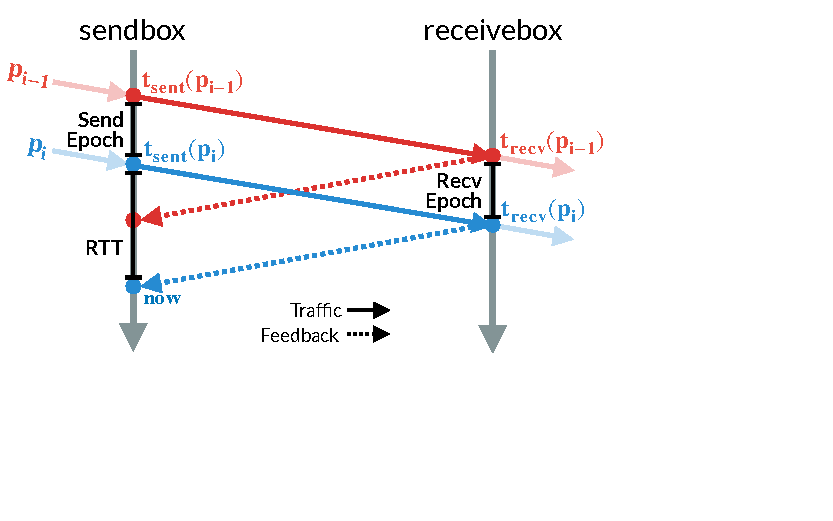
\includegraphics[width=\columnwidth]{img/rate-calculation}
    \caption{Epoch-based measurement calculation}\label{fig:ratecalc}
\end{figure}

Given this method of marking epochs, we can now construct the procedure for computing measurements.

For a given bundle, the \inbox runs the aforementioned function on each packet $p$. Each time
the function returns true, the \inbox updates an epoch data structure that records the packet hash,
which we will call \hptwo\ for the current epoch, 
along with the current time \stwo\ and the \emph{cumulative} number of bytes sent so far, \senttwo. This structure
is sorted by the time the packet was sent, \stwo, but is indexable by the packet hash.

The \outbox runs the same function. Each time it observes a boundary packet, 
it immediately sends a feedback message to the \inbox containing the same information:
the packet hash \hptwo, the time at which it received the packet, \rtwo, and the cumulative number of bytes
\emph{received} up until that point. When the \inbox receives this feedback message at time \atwo, it looks up the
packet hash \hptwo\ in the epoch data structure, which represents the end of the current epoch,
along with the earliest boundary packet still in the data structure, \hpone\ which represents the start
of the current epoch. It now has all of the information necessary to calculate one sample of the following:
\begin{subequations}
    \begin{align}
        RTT &= &now - s_2 \\
        send\_epoch\_duration &= &s_2 - s_1\\
        recv\_epoch\_duration &= &r_2 - r_1\\
        bytes\_sent\_in\_epoch &= &bytes\_sent\ at\ s_2 &\ - \\
                                    &&bytes\_sent\ at\ s_1&\notag\\
        bytes\_rcvd\_in\_epoch &= &bytes\_rcvd\ at\ r_2 &\ - \\
                                &&bytes\_rcvd\ at\ r_1\notag\\
        send\_rate &= &\frac{bytes\_sent\_in\_epoch}{send\_epoch\_duration}\\
        recv\_rate &= &\frac{bytes\_rcvd\_in\_epoch}{recv\_epoch\_duration}
    \end{align}
\end{subequations}
%(Note $bytes\_rcvd\_in\_epoch$ can also be interpreted as the number of bytes
%acknowledged for that epoch, which is a common signal used by many conestion
%control algorithms.)
Finally, it clears all marked packets preceeding \ptwo\ leaving \ptwo\
to be the start of the next epoch.


\subsection{What About Lost Packets?}
\label{s:measure:loss}
This method is robust to the loss of boundary packets between the inbox and outbox.
Suppose the inbox sees boundary packets $p_1, p_2, p_3$, but $p_2$ is lost after passing through
the inbox so the inbox only receives feedback for $p_1$ and $p_3$. Upon receiving $p_1$, 
the inbox will truncate its data structure up until $p_1$. Upon receiving $p_3$, he inbox 
looks up the oldest remaining boundary packet, $p_1$, and considers that the beginning of the epoch.
As a result, the epoch is longer than intended, but no measurements are lost or corrupted. 
The same argument applies to the loss of feedback messages. 
The key here is that the \inbox actually calculates both the send and receive epoch based on information
from the \outbox rather than the \outbox deciding what consitutes an epoch on its own. 


\subsection{Choosing The Epoch Size}
\label{s:measure:epoch}
How do we choose the number of packets that should be in each epoch?
In 3.1, we assumed a fixed epoch size of $N$ packets.
However, in practice, the epoch must be a function of the sending rate.
If the epoch size is too small relative to the rate,
the epochs will be easily influenced by bursts and thus the measurements will be highly variable
and not useful.
If the epoch size is too large relative to the rate, the congestion control algorithm will not
receive feedback frequently enough to respond promptly to changing network conditions. 
As shown in prior work, congestion control algorithms can behave properly even if their
signals are only updated roughly once per RTT~\cite{ccp-hotnets}.
Setting the epoch size equal to our estimate of the number of packets currently inflight 
(our current sending rate multipled by our current esimate of the RTT) will yield roughly
one epoch and thus a new set of measurements once per RTT.

Since the rate and thus the number of inflight packets is continuously changing over time,
we need to continually update the epoch size. Rather than using exactly the number of inflight
bytes, we round the value down to the nearest power of two so that the new epoch size is
always a multiple of the old one and thus will be compatible. 

For examaple, \fc{is an example necessary?}
if the inbox is marking every 256 packets
and the outbox is marking every 512 packets, 
the inbox is just marking a super set of the outbox packets, 
so it is effectively equivalent to them both marking every 512 packets.
    
\subsection{Microbenchmarks}
\label{s:measure:microbench}
    \fc{Maybe this fits better in eval}

    How well do our estimates match the actual signals? In Figure X, we sample a two minute segment from 
    one experiment in our evaluation section and plot the \inbox's estimated values 
    of the RTT and receieve rate compared to the actual RTT and the rate of packets leaving 
    the bottleneck router over time. We find, \fc{...}. The absolute difference between the values
    across time is 

    More generally, we compute the total absolute difference beween the estimated and actual values over the
    course of all experiments in our evaluation, and plot the distributution in Figure Y.
    
\subsection{Limitations}
\subsubsection{Re-Ordering}
\label{s:measure:limitation:reorder}
Earlier we ignored re-ordering of packets between the \inbox and \outbox. However, if packets
are re-ordered, the \inbox and \outbox will observe a different view of the same epoch.
For example, consider packets numbered 1 to 20, where 10 is a boundary packet. The \inbox observes
10 packets in each epoch: [1,10] in epoch 1 and [11,20] in epoch 2. 
However, suppose packet 7 is delayed and arrives after packet 10. The \outbox will observe 9
packets in epoch 1 and 11 packets in epoch 2. 
Spurious re-ordering can be compensated by using an EWMA across epochs rather than the raw values
calculated at each epoch. If there is persitent re-ordering, it may be necessary to add a constant 
value to either the send or receive rate to compensate.

\subsubsection{Suitable Algorithms}
\label{s:measure:limitation:algs}
The set of measurements we obtain are sufficient for most rate-based algorithms, but may not be 
suitable for traditional window-based algorithms which require low-level metrics such as 
the number of inflight packets or number of packets lost. Although it should be possible
to compute these from the measurements we already collect in an ideal scenario, they would easily
break in the presence of network anomilies such as re-ordering. Thus, we leave the development
of robust signals for window-based algorithms to fuure work. 
Thus, \name currently operates best with rate-based algorithms such as BBR, Nimbus, or Copa~\cite{bbr,nimbus,copa}.
